\chapter{Evaluation}
\label{sec:eval}

\todo{how realistic is the simulation?}
\todo{which properties can be modelled well, which can't?}
\section{Testing with Joystick}


In order to evaluate, at an early stage, how flyable and responsivee to external commands the VREP Quadcopter was, and how reliable the communication link between the V-REP and the Ivy-Bus system is, a Hardware-in-the-loop (HIL) set-up was build. \ref{fig:finkenHIL} shows the HIL set-up, consisting of a joystick, which is attached on the Ivy-Bus and controls the V-REP Quadcopter.


\begin{figure}[h!]
 \begin{center}
  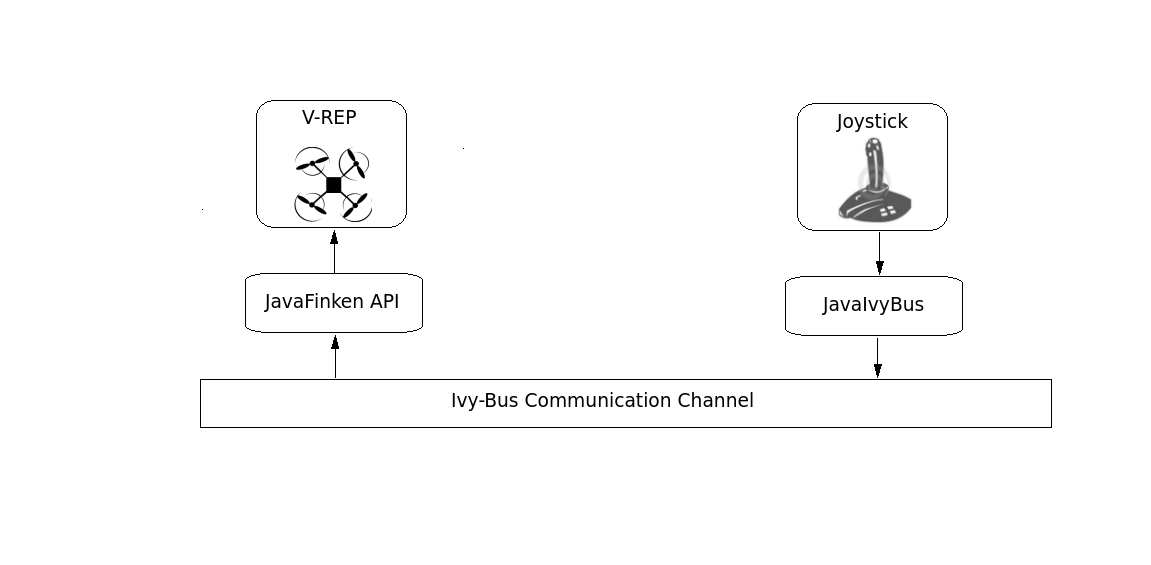
\includegraphics[scale=0.5]{FinkenHIL.png}
 \end{center}
  \caption{Finken Hardware-in-the-loop\label{fig:finkenHIL}}
\end{figure}

The HIL evaluation was implemented as a separate project - \textit{JavaFinkenSimHil}. It uses the Java external library \href{https://java.net/projects/jinput}{JInput} for reading the inputs from the joystick. The already created \textit{JavaIvyBus} module, which was discussed in \ref{sec:ivyBusImplementation}, is used to connect the Joystick to the Ivy-Bus. \\
The \textit{Joystick} class has as a local variable the class \textit{JoystickBusNode}, which extends the abstract \textit{AbsIvyBusNode}, thus being able to communicate on the common Ivy-Bus network. \\
The \textit{Joystick} class polls the data from the Joystick device at 50 Mhz and sends them to the \textit{JoystickBusNode}, which on the other hand encapsulates the data in 
a FINKEN\_ROTORCRAFT\_FP message and publishes it on the bus. \\ 
The FINKEN\_ROTORCRAFT\_FP is the message that the real Quadcopter uses to publish its pitch, yaw and roll angles. Since the Joystick fakes the real Quadcopter, the JavaFinkenApp receives the message as if coming from the real one, thus not even a single line of code had to be changed in the JavaFinkenApp, in order to use the HIL evaluation. \\

As a result of the evaluation we came to the following conclusions:

\begin{itemize}
\item{The controlling of the Quadcopter was very precise and accurate. We ware able to make any manoeuvre and flight path as desired. \\ When flying with the Joystick, one can get a real feeling
of the Quadcopter flight dynamics and behaviour}.

\item{We experienced challenges with keeping the Quadcopter at a level height, using the throttle levers of the Joystick. It turned out, that keeping a level height was a matter of eye-hand coordination. \\
Even the slightest change to the thrust when hovering resulted in a strong accelaration in $z$-axis. Even if this behaviour corresponds to the real quadcopter, we identified it as a problem, as the hover thrust of the real quadcopter changes during flight time with the battery voltage. As a result, we decided to tune the throttle response of the virtual Quadcopter with a logistic curve as described in \ref{equ:logistic}}.

\end{itemize}

\section{Speed}


\todo{communication delay}
\begin{itemize}

\item{mean delta t between sent messages, compare with the configured message frequency}
\item{ run this with two or multiple quadrocopter}
\item{latency of JAVA link}
\end{itemize}


\todo{vrep simulation speed}
\todo{run vrep on the 10core computer in the lab, look at mean execution time}
\todo{add multiple copter}


\section{Accuracy}
\begin{figure}
\begin{center}
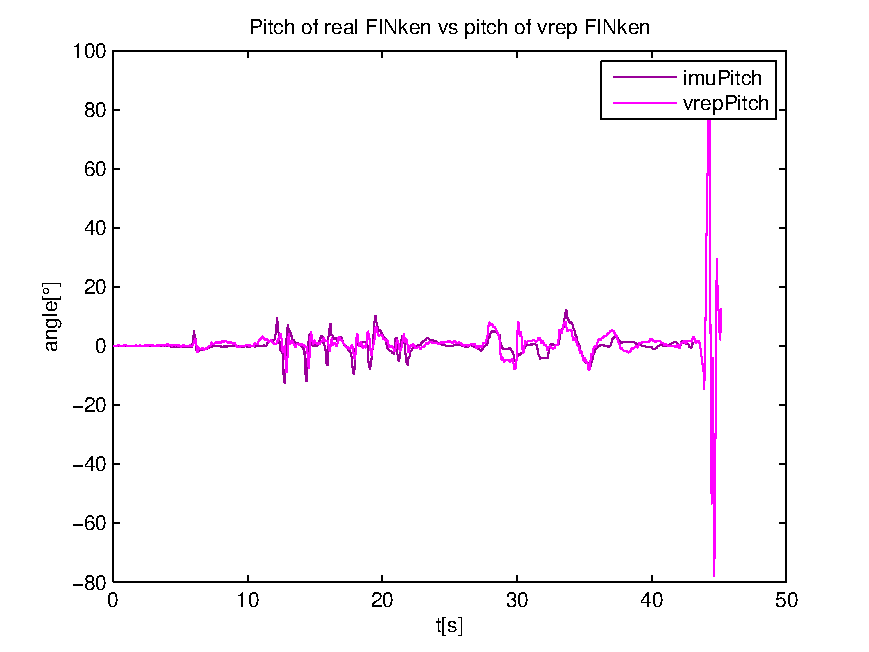
\includegraphics[width=\textwidth]{pitch}
\caption{Euler angles of simulated FINken and real FINken}
\label{pic:pitchResponse}
\end{center}
\end{figure}
\begin{figure}
\begin{center}
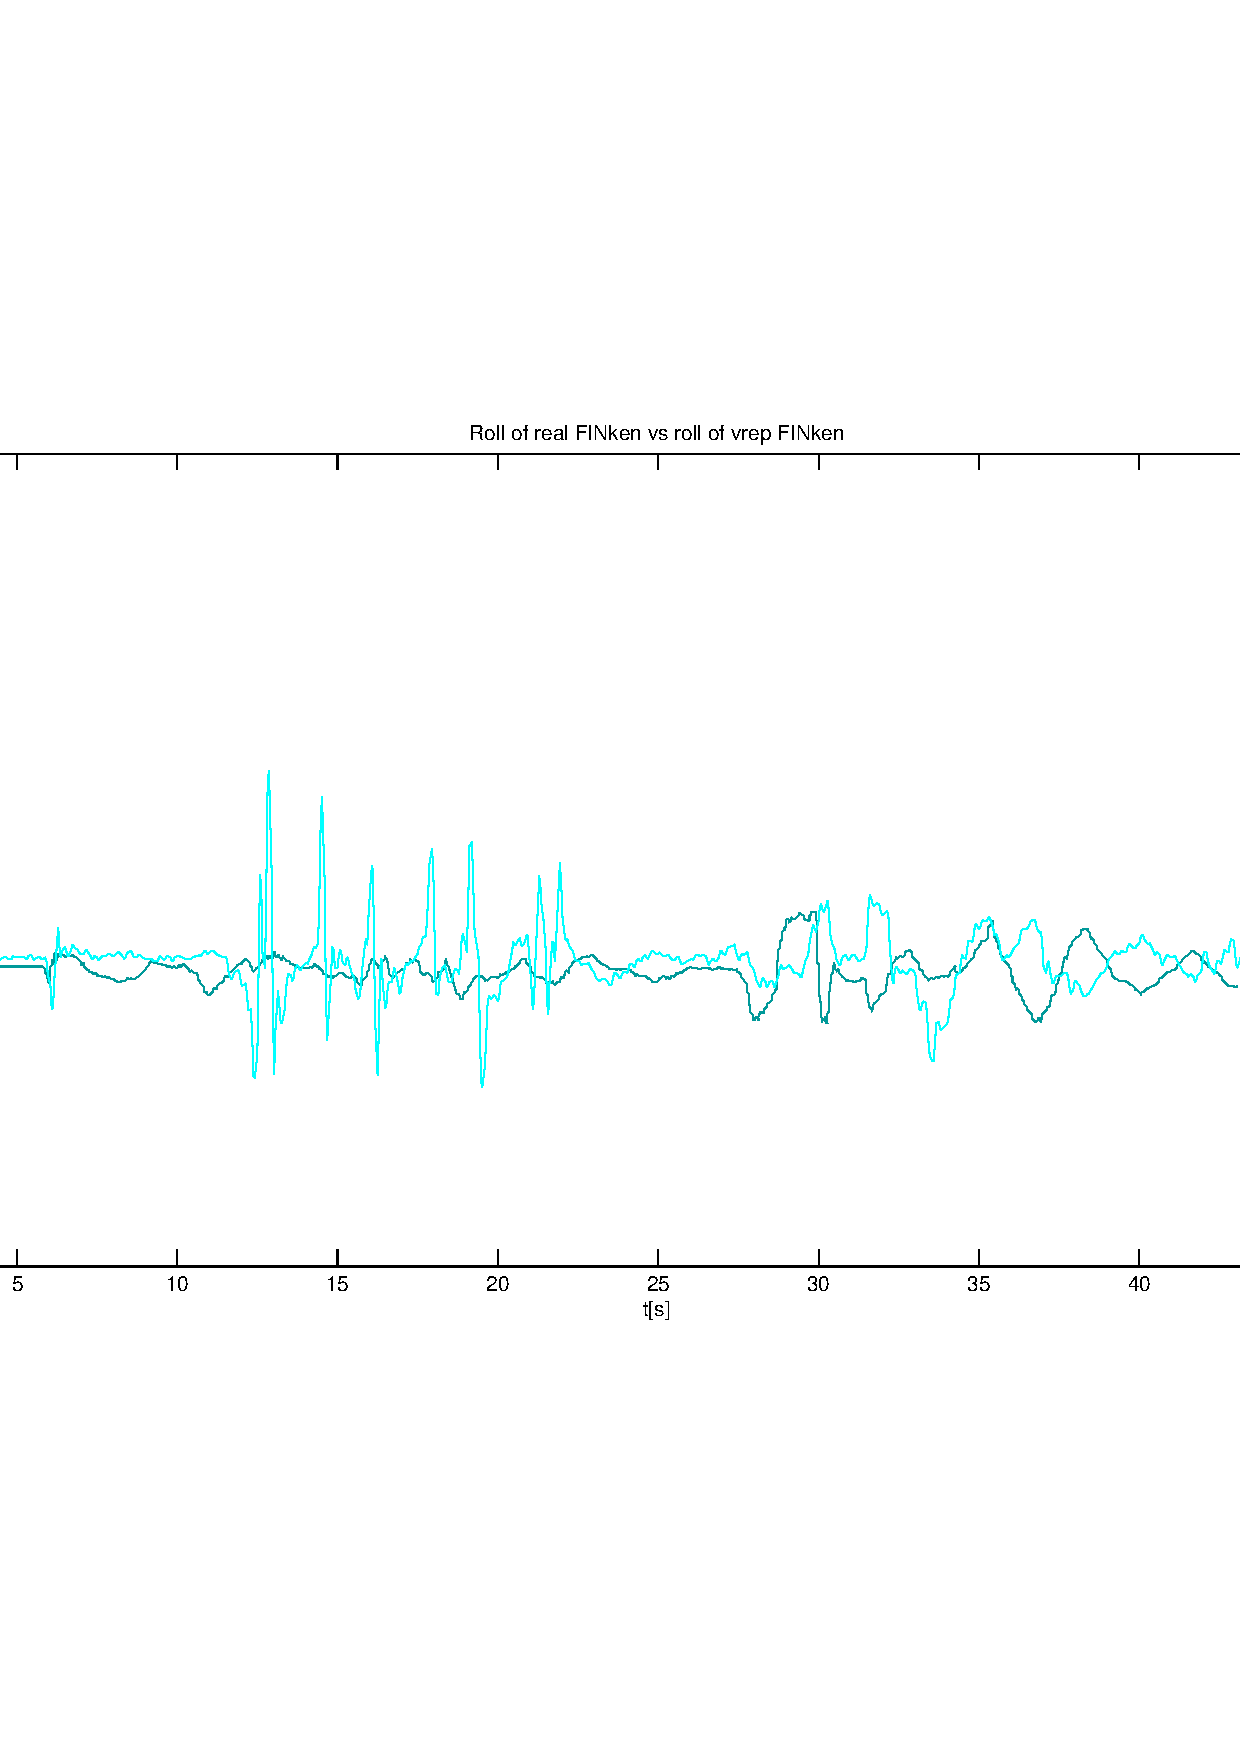
\includegraphics[width=\textwidth]{roll}
\caption{Euler angles of simulated FINken and real FINken}
\label{pic:rollResponse}
\end{center}
\end{figure}
\todo{explanation for roll spikes: vreps internal handling of shapes; maybe copter and "IMU" are not moved at the same time? }
\todo{filter values? }
\begin{itemize}
\item{plot graph of euler angles}
\item{highlight start of drift, other interesting elements?}
\item{plot difference between graphs}
\end{itemize}
\todo{path of quadcopter}
\begin{itemize}

\item{using Medusa positioning system}
\item{shortly explain limitations/problems with the system}
\item{results are not perfect, but it is what is available}
\item{compare scatter plots of real and virtual quadcopter positions}
\end{itemize}

Eventually we wanted to evaluate to what extend the path of the flying quadrocopter matches the path of the simulated quadcopter.

\begin{itemize}
\item{stability}
\item{time that both copter stay inside the arena}
\item{what happens when copter start to drift away?}
\item{maybe show angular movement plot at this time to find explanation there}
\end{itemize}


% example for including picture
%\begin{figure}
%\begin{center}
%\includegraphics[width=\textheight,angle=90]{SimulinkLibArchitect}
%\caption{Aufbau der Conqat Simulink Library}
%\label{slLibArch}
%\end{center}
%\end{figure}
%\begin{figure}
%\begin{center}
%\includegraphics[width=\textwidth]{archDoc}
%\caption{Aufbau des Software-Prototypen}
%\label{pic:saProto}
%\end{center}
%\end{figure}



% example for code listing
%\begin{lstlisting}[caption=Metric-Interface]
%interface Metric {
%/**
% * @return the  value of the metric as it is defined 
% * for the block/architecture and all its subblocks
% */
%    public double getGlobalValue();
%/**
% * @return the worst value of the metric among the 
% * block/architecture and all its subblocks
% */
%    public double getWorstValue();
%/**
% * @return the block with the worst value of the 
% * metric among the block/architecture and all its subblocks
% */
%    public ArchitectureBlock getMaxBlock();
%/**
% * @return a list of all values of the metric for the 
% * block/architecture and its subblocks
% */
%    public double[] getAllBlockValues();
%}
%\end{lstlisting}
%
%
%\begin{lstlisting}[caption=Metric-Interface, label=lst:filter]
%/**
%* disables all subBlocks that are masked in the simulink 
%* Model and have no input
%* @param currentBlock
%*/
%void maskedZeroInDisable(ArchitectureBlock currentBlock){
%   for (ArchitectureBlock subBlock :
%  currentBlock.getSubBlocks()){
%      if (subBlock.getInPorts().isEmpty() && 
%     subBlock.hasAttribute("MaskEnableString")){
%         subBlock.disable();
%      }
%      maskedZeroInDisable(subBlock);
%   }
%}
%\end{lstlisting}
